\pagebreak
\section{\stmt{WENN} Funktion}

$$ \text{\stmt{WENN(\syntax{Bedingung}; [\syntax{Dann\_Wert}]; [\syntax{Ansonsten\_Wert}])}}$$

	\begin{figure}[H]
		\centering
			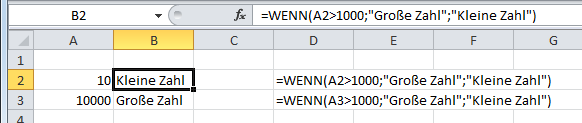
\includegraphics[scale=0.7]{images/wenn_1b}
			\caption{\stmt{WENN} Funktion}
		\label{fig:wenn}
	\end{figure}


Die \stmt{WENN} Funktion liefert in einfachster Form einen Wert zurück. Wenn die \syntax{Bedingung} als WAHR ausgewertet wird, liefert sie den \syntax{Dann\_Wert}, wird sie als FALSCH ausgewertet liefert sie den \syntax{Ansonsten\_Wert}.


Jede \stmt{WENN} Funktion, auch eine verschachtelte, wird automatisch beendet, wenn ein Zweig durchlaufen wird. \stmt{WENN} Funktionen können bis zu 64-fach ineinander verschachtelt werden. Achten Sie bei verschachtelten \stmt{WENN} Funktionen, dass Ihre numerischen Abgrenzungen in den Bedingungen einer logischen Abfolge gleichen.

Im untenstehenden Beispiel ist eine verschachtelte \stmt{WENN} Funktion dargestellt. Ist das Alter mindestens 65 Jahre, dann wird "`ALT"' angezeicht, ist es das nicht, wird danach geprüft, ob das Alter zumindest 35 Jahre ist. Ist das zutreffend, wird "`MITTEL"' angezeigt. Ist die Person unter 35 Jahren, dann wird "`JUNG"' ausgegeben.

	\begin{figure}[H]
		\centering
			%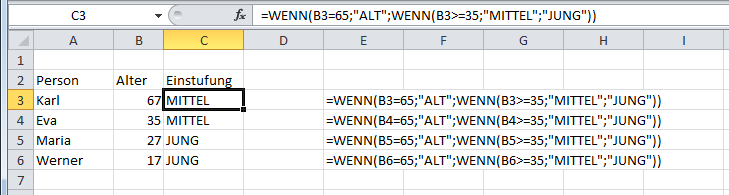
\includegraphics[width=16cm]{images/wenn_verschachtelt_b}
			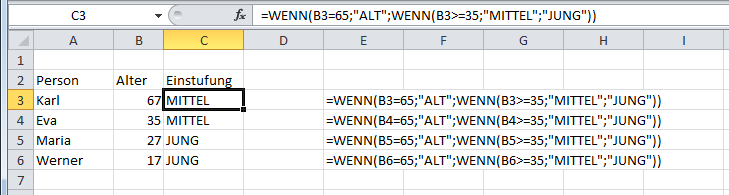
\includegraphics[scale=0.7]{images/wenn_verschachtelt_b}
		\caption{Verschachtelte \stmt{WENN} Funktion}
		\label{fig:wenn_verschachtelt}
	\end{figure}

\begin{lightbulbbox}
Grundsätzlich gilt die Merkregel:\\
Numerische Grenzen von großem nach kleinem Wert immer mit $>$ oder $>=$\\
Numerische Grenzen von kleinem nach großem Wert immer mit $<$ oder$<=$
\end{lightbulbbox}
